% TO-DO:

\documentclass[orivec]{llncs}
\usepackage{graphicx}
\usepackage{float}
\usepackage[most]{tcolorbox}% for wrapping example in color box
\usepackage{wrapfig}		% wrap figure beside text, used in example
\usepackage{tikz-cd}		% commutative diagrams
% \usepackage{amsfonts}
\usepackage[normalem]{ulem}	% underline with line breaks: /uline
\usepackage{enumitem}       % for using (A),(B),(C) in items...
\usepackage{amsmath}		% for "cases"
\usepackage{amsfonts}		% for frakur fonts
\usepackage{mathrsfs}		% for curly "E" error symbol
\usepackage{amssymb}		% for \multimap, \updownarrow, \bigstar
\usepackage{turnstile}		% longer turnstiles
\usepackage{sectsty}		% change section color
\usepackage{hyperref}		% refs, links become clickable
\usepackage{url}			% for urls in bibliography
\usepackage[normalem]{ulem} % underline unbroken with \uline
\usepackage[numbers,sectionbib]{natbib}% if we use \package{url} we need to use natbib style
\usepackage{unicode-math}

%\def\chinchin{yes}          % ********** 用中文 *********
% *************** Delete when not using Chinese or colors **********************
\ifdefined\chinchin
\usepackage{xeCJK}
\setCJKmainfont[BoldFont=SimHei,ItalicFont=KaiTi]{SimSun}
\newcommand{\cc}[2]{#1}
\else
\newcommand{\cc}[2]{#2}
\fi
\usepackage{color}
%\newcommand{\emp}[1]{\textbf{\textcolor{blue}{#1}}}
\newcommand{\emp}[1]{\textbf{#1}}

\sectionfont{\color{blue}} 
\subsectionfont{\color{blue}} 
\subsubsectionfont{\color{blue}} 
\definecolor{green}{rgb}{0,0.7,0}
\definecolor{grey}{rgb}{0.95,0.95,0.95}

\usepackage{geometry}		% change paper size
\geometry{
  a4paper,         % or letterpaper
  textwidth=18cm,  % llncs has 12.2cm
  textheight=27cm, % llncs has 19.3cm
  heightrounded,   % integer number of lines
  hratio=1:1,      % horizontally centered
  vratio=2:3,      % not vertically centered
}
\usepackage[fontsize=13pt]{scrextend}

\newcommand{\tikzmark}[1]{\tikz[overlay,remember picture] \node (#1) {};}

\newcommand{\vect}[1]{\boldsymbol{#1}}
\newcommand*\sigmoid{\vcenter{\hbox{
\includegraphics{sigmoid.png}}}}
\newcommand*\rectifier{\vcenter{\hbox{\includegraphics{rectifier.png}}}}
\newcommand*\KB{\vcenter{\hbox{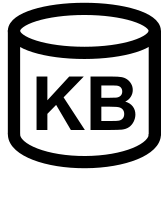
\includegraphics{KB-symbol.png}}}}
\newcommand*\KBsmall{\vcenter{\hbox{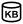
\includegraphics{KB-symbol2.png}}}}
\newcommand*\NN{\vcenter{\hbox{
\includegraphics{NN-symbol.png}}}}
\newcommand*\Graph{\vcenter{\hbox{\includegraphics{../graph-symbol.png}}}}
\newcommand*\Hypergraph{\vcenter{\hbox{\includegraphics{../hypergraph-symbol.png}}}}
\newcommand*\Tree{\vcenter{\hbox{\includegraphics{../tree-symbol.png}}}}
\newcommand*\NewSym[1]{\vcenter{\hbox{\includegraphics{#1}}}}
\newcommand{\dashh}{\textemdash~}
\newcommand{\english}[1]{\mbox{\textit{#1}}}
\newcommand{\tab}{\hspace*{2cm}}

% ***** Boxed variables inside math equations
% \newcommand*{\boxedcolor}{black}
\makeatletter
% \renewcommand{\boxed}[1]{\textcolor{\boxedcolor}{%
% \fbox{\normalcolor\m@th$\displaystyle#1$}}}
% \setlength{\fboxsep}{1pt}
\renewcommand{\boxed}[1]{\fbox{\m@th$\displaystyle\scalebox{0.9}{#1}$} \,}
\makeatother

\overfullrule=0mm

\newsavebox{\MyName}
\savebox{\MyName}{
\includegraphics[scale=0.6]{YKY.png}}

\title{My problem}
% \titlerunning{Direct knowledge injection}
\author{\usebox{\MyName} (King-Yin Yan)
% \\ \footnotesize{General.Intelligence@Gmail.com}
%\and
%Ben Goertzel
%\and
%Juan Carlos Kuri Pinto
}
\institute{General.Intelligence@Gmail.com}
\date{\today}

\begin{document}
\let\labelitemi\labelitemii

\maketitle

\noindent
\makebox[\linewidth]{\small \today}

\setlength{\parindent}{0em}
\setlength{\parskip}{2.8ex plus0.8ex minus0.8ex}
% \setlength{\parskip}{2.8ex}

%\begin{abstract}
%\end{abstract}

%\begin{keywords}
%reinforcement learning, control theory, deep learning, cognitive architecture
%\end{keywords}

%\setcounter{section}{-1}

The problem I want to solve is to combine these 2 paradigms:
\begin{itemize}
	\item  reinforcement learning (also known as dynamic programming)
	\item  logical reasoning
\end{itemize}

\section*{Part 1}

The first part is pretty standard:  It consists of a dynamical system:
\begin{equation}
x_{t + 1} = F(x_t, u_t)
\end{equation}
where $u$ is the \textbf{control}.  The problem is to seek an optimal trajectory of $x_t$.  In artificial intelligence, $x$ is the \textbf{mental state} of an intelligent agent, $F$ is its \textbf{knowledge-base}.  The reward at state $x$ is given by $L(x)$ where $L$ corresponds to the \textbf{Lagrangian} in the Hamiltonian formulation.  In other words we are trying to maximize the \textbf{action} which is the time integral of the Lagrangian:
\begin{equation}
\boxed{action} \quad A = \int L(x(t)) dt
\end{equation}
The optimality condition is given by the \textbf{Hamilton-Jacobi equation}, its discrete version is called the \textbf{Bellman equation}.  We are not just trying to find the optimal trajectory $x_t$, but we are also \textit{learning} $F$ itself, because $F$ represents the knowledge of the agent and is modifiable.

We use a (deep) neural network to represent $F$, that is to say:
\begin{eqnarray}
& \mbox{\footnotesize \textbf{weight} matrix } \tikzmark{weightMatrix} \mbox{\footnotesize for each layer} \quad \quad \mbox{\footnotesize total \# of layers} \tikzmark{numLayers} \nonumber \\
\nonumber \\
& \vect{x}_{t+1} = F(\vect{x}) = \sigmoid(W_1 \tikzmark{wa} \sigmoid(W_2 \tikzmark{wb} ... \sigmoid( W_L \tikzmark{wc} \tikzmark{L} \; \vect{x} )))
\begin{tikzpicture}[overlay,remember picture]
\draw (weightMatrix.center) +(17pt,-5pt) -- ([shift={(-10pt,10pt)}]wa.center);
\draw (weightMatrix.center) +(21pt,-5pt) -- ([shift={(-10pt,10pt)}]wb.center);
\draw (weightMatrix.center) +(33pt,-5pt) -- ([shift={(-10pt,10pt)}]wc.center);
\draw (numLayers.center) +(-20pt,-5pt) -- ([shift={(-2pt,6pt)}]L.center);
\end{tikzpicture}
\end{eqnarray}

So our dynamical system is a deep neural network joined from end to end to form a loop, also called a \textbf{recurrent} neural network.  The dynamical state $x$ changes from each iteration (ie, 1 pass) of the neural network.

So far, all this is pretty standard.  It belongs to the currently very hot research topic of ``deep reinforcement learning''.

\section*{Part 2}

在逻辑中,$\Psi_1 \vdash \Psi_2$ 代表 \textbf{逻辑推导},其中 $\Psi_1$ 是\textbf{前提},$\Psi_2$ 是\textbf{结论}。 对应於 Boolean lattice 可以记作:
\begin{equation}
\boxed{logic} \quad \Psi_1 \vdash \Psi_2 \quad \Leftrightarrow \quad \Psi_1 \le \Psi_2 \quad \boxed{lattice}
\end{equation}
(注意方向相反,是惯例)

我的目的是: 令 神经网络 $F$ 做 $\vdash$ 的工作,换句话说 $F$ approximates $\vdash$。

$F$ 的作用是在 Boolean lattice 中\textbf{向下移一步},对应於逻辑中的\textbf{一步推论} (single-step deduction)。 

我的问题是:  既然 $F$ 有这 lattice monotone automorphism 的结构,那么 $F$ 作为一个 neural network,它的 learning algorithm 应该可以\textbf{加快}。  换句话说,可以\textbf{交替}使用 Bellman update (for Part 1) 和 ``lattice update'' (for Part 2),similar to the \textbf{Method of Alternating Projections} of convex sets.  因为我们需要同时符合 Parts 1 and 2 的两个条件。  在机器学习的术语中,我们的 search space 缩小了 (dimensionality reduction),因为原本的 search space 是 $F$ 的 function space,新的 search space 是 quotient 了 Boolean lattice 的结构。

神经网络 $F: V \rightarrow V$ 作用在 vector space 上,但 $\vdash: L \rightarrow L$ 作用在 Boolean lattice 上,所以需要将 Boolean lattice represent 到 vector space 上,亦即 $\rho: L \rightarrow V$。 

Satisfying the following commutative diagram:
\begin{itemize}
	\item $L$ 代表 Boolean lattice, with order relation $\ge$.
	
	\item $f: L \rightarrow L$ 是 monotonous automorphism,即 $f(a) \ge f(b)$ if $a \ge b$.
	
	\item $V$ 是 vector space, $\rho$ is a representation $\rho: L \rightarrow V$.
	
	\item $F$ 是在 $\rho$ 之下 保持 $\ge$ 关系 的映射,亦同时是上一节的 neural network function。
\end{itemize}
\begin{equation}
\begin{tikzcd}
L \arrow{r}{f} \arrow[swap]{d}{\rho} & L \arrow{d}{\rho} \\
V \arrow{r}{F} & V
\end{tikzcd}
\end{equation}

但我暂时不清楚 $\rho$ 的做法,和 $F$ 如何 construct。

\bibliographystyle{unsrtnat} % or number or aaai ...
\bibliography{AGI-book}

\end{document}
